\documentclass[12pt,a4paper]{scrartcl}

\usepackage[english]{babel}
\usepackage[T1]{fontenc}
\usepackage{graphicx, subfig}
\usepackage[document]{ragged2e}
\usepackage{lmodern}
\usepackage{color}
\usepackage{amsmath}
\usepackage{graphicx}

% Für Verwendugn von Utnerstrichen ohne Escaping
\usepackage{underscore}

% Für Referenzen mit eigenem Text
\usepackage{hyperref}

% Für Codeblöcke
\usepackage{listings}

% Für Verwendung von Farben
\usepackage[usenames,dvipsnames,svgnames,table]{xcolor}

% Für Verktor-Pfeile
\usepackage{esvect}

% Für Größe der Seitenränder
\usepackage[margin=1in,footskip=0.5in]{geometry}

% Für Tabellen über Seiten hinweg
\usepackage{longtable}

% Für Header and Footer
\usepackage[automark]{scrpage2}

% Für Bildunterschriften
\usepackage[aboveskip=2pt]{caption}

% Formatierung für Hyperref-Referenzen
\hypersetup{
	colorlinks,
	linkcolor={blue!50!black},
	citecolor={blue!50!black},
	urlcolor={blue!80!black}
}

% Generelle Formatierung für Code-Blöcke
\lstset{ %
	columns=fullflexible,
	keepspaces=true,
	frame=single,
	breaklines=true,
	breakautoindent=true,
	gobble=0,
	tabsize=2,
	belowskip=0pt
}

% Formatierung für Pseudo-Code
\lstdefinelanguage{PSEUDO} 
{ 
	xleftmargin=0pt, 
	xrightmargin=0pt,
	basicstyle=\small\ttfamily\color{Black},
	morekeywords={for, each, if, else},	
	keywordstyle = {\color{Orange}},
	sensitive=false,
	morecomment=[l]{//},
	morecomment=[s]{/*}{*/},
	morestring=[b]"
}

\title{Rendering and Manipulating Quad Meshes and Bezier Surfaces}
\author{Fabian Niehaus, Tuyet Nguyen}
\date{May 14, 2018}

\makeatletter

%% Generelle Kopf- und Fußzeilendefinition
\pagestyle{scrheadings}
%\automark[section]{subsection} 
\clearscrheadfoot
\ihead[]{\@title}
%\ohead[]{\rightmark}
\ifoot[]{\@author}

\begin{document}

\begin{titlepage}
	\centering
	\ \\[2cm]
	{\huge\textbf{\@title}} 
	\\[3cm]
	\large
	\textbf{Field of study:} Media informatics \\
	\textbf{Semester:} 4
	\\[2cm]
	\textbf{Date}: \@date
	\\[2cm]
	\textbf {Authors:}
	\\Fabian Niehaus
	\\Tuyet Nguyen
\end{titlepage}

\newpage
%% Seitezahl auf 0 setzen
\setcounter{page}{0}
\tableofcontents
\newpage
\listoffigures

\newpage
%% Seitennummern einblenden
\ofoot[]{\pagemark}
\normalsize

\section{Abstract}
In this project we will build a C++ application that can read, render and write quad meshes and apply the Catmull-Clark subdivision algorithm. It will also be able to read and compute Bezier surfaces and create rotational sweep surfaces from Bezier curves. We will use QT Creator for programming, QT for window management and OpenGL for 3D rendering.

\section{Realisation}

\subsection{Creating an interface with QT}
First off, we create a new QT widget application. This allows us to use QT Creators design feature to set up our application's interface. A new QOpenGLWidget is placed and will be used as a placeholder for a new custom class inheriting QOpenGLWidgets functionality. This class, called OGLWidget, needs to implement the following methods: initializeGL (for setting up OpenGL), paintGL (for doing the actual rendering), resizeGL (for handling resizes of the display window). Additionally, the functions SetMaterialColor and InitLightingAndProjection\footnote{Taken from Prof. Dr. Martin Hering-Bertrams OpenGL_Example} are used.

\subsection{Creating the data structure}
The data structure is separated in different classes. \\
The basic class "Vertex" contains the three coordinates and the valence. \\ 
The basic class "Quad" contains the indices of four vertices, the indices of four adjacent quads, the index of its face vertex and the four indices of its edge vertices, the latter two being calculated in the process of the Catmull-Clark subdivision. \\
Logic and data regarding the computation of quad meshes is stored in a seperate class, as are Bezier surfaces and rotational sweep surfaces. \\
In order to allow for easier use of a two dimensional matrix of vertices, a wrapper class containing a two dimensional vector of vertices is introduces. \\

\subsection{Reading the data from a file}
\subsubsection{Quad mesh}
After creating the required data structure, a method for reading the vertices and faces from an .obj file is implemented. For this project we can assume that every face is a quad. The distinction between a vertex and a quad is made by the first letter in the line, a "v" for vertices and an "f" for quads. \\
Each line is read, and depending on the first letter a new Vertex or Quad is created and pushed to the respective vector.
\subsubsection{Bezier surface}\label{read-bezier}
The initial surface data for Bezier calculations is stored in a data format that separates the x, y and z coordinates in different blocks. Each block is read and its values stored in a temporary matrix. After alls blocks have been read, a matrix of vertices is created from this data. This matrix is then used to create quads. Vertices and Quads are stored for further use within the object.

\subsection{Rendering Quad meshes}
Depending on the desired way of rendering the object, different draw methods are implemented. These methods are then being called from the paintGL() function.

\subsubsection{Rendering as a wireframe}
At first, we want to render the object a wireframe without any specific lighting or normals. The method drawLines() implements this by going through the list of quads and connecting every two points that are next to each other, using GL_Lines. Every line needs two points as input, so every point is mentioned twice considering we need 4 lines per quad in total.

\subsubsection{Rendering as a solid}
After drawing the object as a wireframe we want to draw it as a solid cube with lighting. This is being achieved in the method drawQuads() which once again iterates over the list of quads. This time using GL_Quads, the four vertices of a quad are connected and the area inbetween is filled. The normal vector for this is calculated using the cross product of the two diagonals vectors.

\subsection{Calculation the vertex valence}
After making sure that the meshes are read and rendered correctly, the vertex valence is to be calculated. Vertex valence in this context means how many edges a single vertex is connected to. To calculate this, the following algorithm is used:


\begin{lstlisting}[language=PSEUDO]
for each vertex 
	for each quad 
 		for each vertex of this quad
   			if index of both vertices is equal 
   				increase valence of vertex by 1
\end{lstlisting}
\captionof{figure}{Calculation vertex valence (pseudo code)}

\subsection{Determining adjacent quads}
In order to determine each quads adjacent quads (or neighbors for short), we need to check if it has a shared edge with another quad. This is calculated by comparing if they share two vertices. The algorithm looks as follows:

\begin{lstlisting}[language=PSEUDO]
for each quad
	for i = 0 to 3 // since each quad has 4 vertices
		a = index of vertex at i
		b = index of vertex at (i+1)%4
		for each quad that is not the current one
			compare all vertices to a and b
			if a and b have a match
				add index of quad to current quads list of neighbors at index i 
\end{lstlisting}
\captionof{figure}{Determining adjacent quads (pseudo code)} 

\subsection{Printing the data}
In order to verify the correctness of the results, all data is printed to the console. Additionally, each vertex (now with their valence) and quad (now with its neighbors) is written back to a .obj file.

\subsection{Catmull-Clark-Subdivision}

\subsubsection{Calculating the Face-Mask}
In the first step of the Catmull-Clark-Subdivision process, the so called Face-Mask is calculated. It describes the middle point of each quad. Mathematically speaking, it is the average of the four vertices of the quad:

$$ \vv{f} = \frac{1}{4}*( \vv{v}\textsubscript{0} + \vv{v}\textsubscript{1} + \vv{v}\textsubscript{2} + \vv{v}\textsubscript{3}) $$

This calculation is run for every quad. The resulting vertex is added to the list of vertices, and the index of it is stored within the quad.

\subsubsection{Calculating the Edge-Masks}
In the next step, the four edge masks are calculated. These vertices are the average between two end vertices of an edge and the face vertices of the two quads sharing this egde.\\
The formula for a single one of these points is:

$$ \vv{e} = \frac{1}{4} * (\vv{v}\textsubscript{a} + \vv{v}\textsubscript{b} + \vv{f} + \vv{f}\textsubscript{neighbor}) $$

This calculation is only run once per edge, meaning that only the quad with the lower index calculates the mask. The adjacent quad with the higher index only copies the reference. The following algorithm is used for the entire calculation.
\begin{lstlisting}[language=PSEUDO]
for each i = 0 to (size of quads - 1)
	Q = quad at index i
	for j = 0 to 4
		N = adjacent quad at index j in array of neigbors of Q
		if index of q is smaller than index of N
			calculate the edge mask using the formula explained above
		else
			for k = 0 to 4
				if value at index k of Ns adjacent quads = i
					add Ns edge mask of index k to Qs edge masks at index j		
\end{lstlisting}
\captionof{figure}{Calculating the Edge-Masks (pseudo code)}  

\subsubsection{Calculating the Vertex-Masks}
The last mask calculated is the Vertex-Mask. With this mask every original vertex of a quad is repositioned using the following formula:

$$ \vv{v}\textsubscript{new} = \frac{1}{(n\textsubscript{v})^{2}}*(2 \vv{e}\textsubscript{v\textsubscript{left}} + 2 \vv{e}\textsubscript{v\textsubscript{right}} - \vv{f}\textsubscript{v} +\vv{v} (n\textsubscript{v}(n\textsubscript{v}-3))) $$

The implementation is split into the three following steps:\\
\ \\
1.) Multiply every corner vertex with a product of its valence: $ \vv{v}\textsubscript{new} = \vv{v} (n\textsubscript{v}(n\textsubscript{v}-3)$
\begin{lstlisting}[language=PSEUDO]
for each vertex
	if vertex is corner vertex
		recalculate the vertex using the above formula
\end{lstlisting}
\captionof{figure}{Calculating the Vertex-Masks - step 1 (pseudo code)}  
\ \\
\ \\
2.) Add edge vertices and subtract face vertex from each corner vertex of each quad: $\vv{v}\textsubscript{new} = \vv{v} + 2 \vv{e}\textsubscript{v\textsubscript{left}} + 2 \vv{e}\textsubscript{v\textsubscript{right}} - \vv{f}\textsubscript{v}$
\begin{lstlisting}[language=PSEUDO]
for each quad
	for each corner vertex of this quad
		recalculate the vertex using the above formula
\end{lstlisting}
\captionof{figure}{Calculating the Vertex-Masks - step 2 (pseudo code)}  
\ \\
\ \\
3.) Divide each corner vertex by its valence squared: $ \vv{v}\textsubscript{new} = \vv{v} * \frac{1}{(n\textsubscript{v})^{2}}$
\begin{lstlisting}[language=PSEUDO]
for each vertex
	if vertex is corner vertex
		recalculate the vertex using the above formula
\end{lstlisting}
\captionof{figure}{Calculating the Vertex-Masks - step 3 (pseudo code)}  

\subsubsection{Reconnecting the mesh}
In the final step of the Catmull-Clark-Subdivision every quad is divided into 4 smaller quads. These smaller quads are added to a newvector. After all quads have been subdivided, the original vector storing the quads is overwritten with the new vector storing four times the amout of quads.
\begin{lstlisting}[language=PSEUDO]
for each quad
	for j = 0 to 4
		v0 = corner vertex of the quad at index j
		v1 = edge vertex of the quad at index j
		v2 = face vertex of the quad
		v3 = edge vertex of the quad at index (j-1)%4 //tuned to always be positive
		create new quad with corner vertices v0 - v4 and store it
\end{lstlisting}
\captionof{figure}{Reconnecting the mesh (pseudo code)}  

\subsection{Bezier surface calculation}
In this section, Bezier surface calculation is applied to the surface created when 
\hyperref[read-bezier]{reading the bezier surface}. The calculation for a matrix of dimension 
\textit{m}x\textit{n} uses the following forumla
$$f(s,t) = \sum_{i=0}^{m} \sum_{j=0}^{n} b_ij*B_i^m(s)*B_j^n(t)$$
where s and t are defined within [0;1]. \\
\ \\
B descibes the so called Bernstein polynomial $B_i^n(t) = {n \choose i}*t^i*(1-t)^{n-i}$. \\
\ \\
A resolution describing the amount of new vertices created is introduced. In this case we chose a value of 0.05 meaning 21x21 new points are calculated.
\begin{lstlisting}[language=PSEUDO]
for s = 0 -> 1; increased by resolution {
	for t = 0 -> 1; increased by resolution 
	
		Vertex v = (0, 0, 0)
	
		for i = 0 -> m {
			for j = 0 -> n 
				
				multiply vector at (i|j) with Bernstein 
				polynomials of (i,m,s) and (j,n,t)
					
				add resulting vector to v
		}
		
		store v in new matrix at position (s * resolution | t * resolution)
\end{lstlisting}
\captionof{figure}{Bezier surface calculation (pseudo code)}  

\subsection{Rotational sweep surface calculation}
In this section, a rotational sweep surface is calculated from a single bicubic curve. 
\subsubsection{Cubic bezier curve calculation}
First, Bezier transformation is applied to the two dimensional curve using the formula below:
$$ p(t) = (1-t)^3*p_1 + 3t*(1-t)^2*p_2 + 3t^2*(1-t)*p_3 + t^3*p_4$$
$$t = [0;1]$$
A resolution is of 0.05 is used for t, resulting in 21 new points.
\begin{lstlisting}[language=PSEUDO]
for t = 0 -> 1; increased by resolution
	
	calculate and store new point according to
	the formula above
	
\end{lstlisting}
\captionof{figure}{Cubic bezier curve calculation (pseudo code)}  
\subsubsection{Rotational sweep surface creation}
Using the Bezier curve calculated in the last step, a new surface is created. Since the curve is in two dimensional space we need translate every point into 3D space using the following logic:
$$x_{new} = x$$
$$y_{new} = y * sin(t * \pi)$$
$$z_{new} = y * cos(t * \pi)$$
$$t = [-1;1]$$
Again, a resoultion of 0.05 is used resulting in a total of 21x21 new vertices.
\begin{lstlisting}[language=PSEUDO]
for t = 0 -> 1; increased by resolution
	for i = 0 -> 20 // since there are 21 points
	
		calculate new vertex according to the formula above
		using the vertex at index i as input
		
		store new vertex in matrix at position (t * resolution | i)
\end{lstlisting}
\captionof{figure}{Rotational sweep surface vertex creation (pseudo code)}  
\ \\
\ \\
After calculating the vertices for the new surface, quads are also created in order to draw it using drawQuad().
\begin{lstlisting}[language=PSEUDO]
for i = 0 -> 20 - 1; // since we are also accessing i + 1 and j + 1
	for j = 0 -> 20 - 1;
		
		create new Quad from (
			vertex at (i|j)	
			vertex at (i|j+1)
			vertex at (i+1|j+1)
			vertex at (i+1|j)
		)

		store new Quad
\end{lstlisting}
\captionof{figure}{Rotational sweep surface quad creation (pseudo code)}  

\subsection{Rendering multiple objects in a scene}
In order to render multiple objects within a single scene, the methods glLoadIdentity() and glTranslated() are used.
glLoadIdentity() resets all translation, rotation and color settings everything back to default. glTranslated() allows us to move an object within a scene.
\begin{lstlisting}[language=PSEUDO]
glLoadIdentity(); //reset to default

set the color

glTranslated(); // set the translation

set the object scale (better visibility)

set th initial object rotation

set the constant object rotation

draw the object
\end{lstlisting}
\captionof{figure}{Setting tranlsation, rotation and color for a single object (pseudo code)}  


\section{Results}
\subsection{Number of vertices, faces (quads) and edges after subdivision}

\begin{tabular}{ll}
	Data used: cube.obj & Data used: threehole.obj \\
	\begin{tabular}{|l|l|l|l|}
		\hline
		Subdivisions & Vertices & Faces & Edges \\
		\hline
		0 & 8 & 6 & 12 \\
		\hline
		1 & 32 & 24 & 48 \\
		\hline
		2 & 128 & 96 & 192 \\
		\hline
		3 & 512 & 384 & 768 \\
		\hline
	\end{tabular}
	&
	\begin{tabular}{|l|l|l|l|}
		\hline
		Subdivisions & Vertices & Faces & Edges \\
		\hline
		0 & 64 & 68 & 136 \\
		\hline
		1 & 268 & 272 & 536 \\
		\hline
		2 & 1084 & 1088 & 2176 \\
		\hline
		3 & 4348 & 4348 & 8696 \\
		\hline
	\end{tabular}
	\\
\end{tabular}
\captionof{figure}{Subdivisions, vertices, faces and edges for Cube and Threeholes}


\subsection{Rendering and subdivision}

\begin{center}
	\begin{tabular}{cc}
		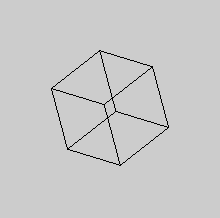
\includegraphics[width=150px, height=150px]{Images/cube-wireframe.png} 
		& 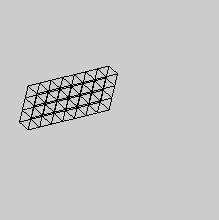
\includegraphics[width=150px, height=150px]{Images/threeholes-wireframe.png}  \\
	\end{tabular}
	\captionof{figure}{Wireframe Cube and Threeholes}
	\ \\
	\begin{tabular}{cc}
		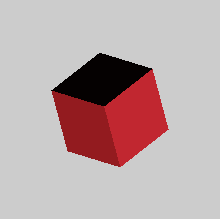
\includegraphics[width=150px, height=150px]{Images/cube-solid.png} 
		& 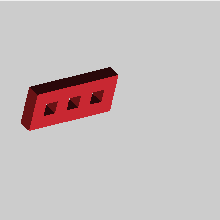
\includegraphics[width=150px, height=150px]{Images/threeholes-solid.png}  \\
	\end{tabular}
	\captionof{figure}{Solid Cube and Threeholes}
	\ \\
	\begin{tabular}{cc}
		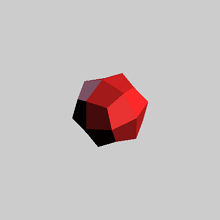
\includegraphics[width=150px, height=150px]{Images/cube-1sd.png} 
		& 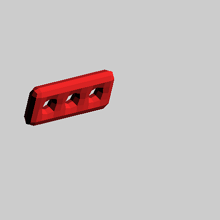
\includegraphics[width=150px, height=150px]{Images/threeholes-1sd.png}  \\
	\end{tabular}
	\captionof{figure}{1 CC-Subdivision Cube and Threeholes}
	\ \\
	\begin{tabular}{cc}
		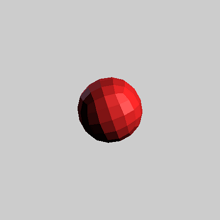
\includegraphics[width=150px, height=150px]{Images/cube-2sd.png} 
		& 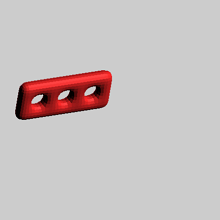
\includegraphics[width=150px, height=150px]{Images/threeholes-2sd.png}  \\
	\end{tabular}
	\captionof{figure}{2 CC-Subdivisions Cube and Threeholes}
	\ \\
	\begin{tabular}{cc}
		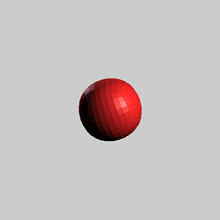
\includegraphics[width=150px, height=150px]{Images/cube-3sd.png} 
		& 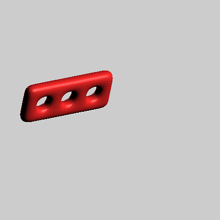
\includegraphics[width=150px, height=150px]{Images/threeholes-3sd.png}  \\
	\end{tabular}
	\captionof{figure}{3 CC-Subdivisions Cube and Threeholes}
	\ \\
	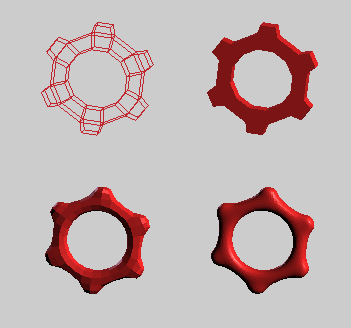
\includegraphics[width=300px, height=300px]{Images/gear-stages.png} 
	\captionof{figure}{Wireframe, Solid, 1 CC and 3 CC Gear}
\end{center}

\subsection{Bezier surfaces}
\begin{center}
	\begin{tabular}{cc}
		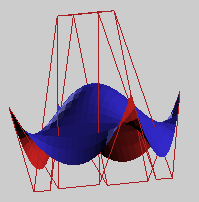
\includegraphics[width=100px]{Images/bezier-01.png} 
		& 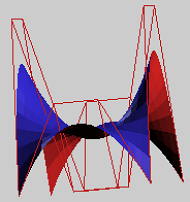
\includegraphics[width=100px]{Images/bezier-02.png}  \\
	\end{tabular}
	\captionof{figure}{Bezier surfaces generated from bezier01 and bezier02}
\end{center}

\subsection{Rotational sweep surfaces}
\begin{center}
		\begin{tabular}{cc}
		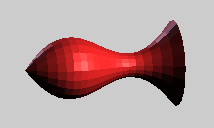
\includegraphics[width=150px]{Images/sweep-01.png} 
		& 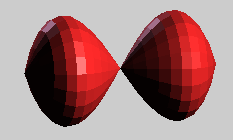
\includegraphics[width=150px]{Images/sweep-02.png}  \\
	\end{tabular}
	\captionof{figure}{Sweep surfaces generated from curve01 and curve02}
\end{center}

\subsection{Multiple objects in single scene}
\begin{center}
	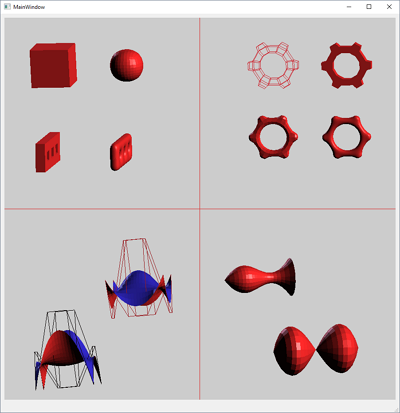
\includegraphics[width=400px]{Images/scene.png} 
	\captionof{figure}{Multiple objects in a single scene}
\end{center}

\section{Conclusion}
We were able to successfully build an application that can read and write any kind of boundary-free quad meshes, render them and perform Catmull-Clark-Subdivision on them. It can also read Bezier curves and surfaces, apply the appropriate calculations and create rotational sweep surfaces from the curves. \\
We gained a deeper understanding of how OpenGL and QT work as well as the mathematics behind the Catmull-Clark-Subdivision, Berzier curves and surfaces and rotational sweep surfaces. We will be able to extend the code for further applications and to reuse parts of it for other purposes.

\section{Acknowledgements}
\begin{itemize}
	\item User Martin B on StackOverflow for supplying the function for always positive modulos in C++
	\item The QT Company, GitHub, the developers of TeXStudio and the developers of MiKTEX for letting us use their software free of charge
	\item Prof. Dr. Martin Hering-Bertram for providing the OpenGL example code for coloring, lighting and projection used in the project
\end{itemize}

\section{References}
\begin{thebibliography}{0} 
	\bibitem{CG18_1}
	Prof. Dr. Martin Hering-Bertram,
	\textit{Lecture CG18_1},
	HSB,
	2018.
	
	\bibitem{CG18_1}
	Prof. Dr. Martin Hering-Bertram,
	\textit{Lecture CG18_2},
	HSB,
	2018.
\end{thebibliography}

\section{Appendices}
\subsection{Input file cube.obj}
\begin{lstlisting}
v  1.0  1.0  1.0
v  1.0  1.0 -1.0
v  1.0 -1.0  1.0
v  1.0 -1.0 -1.0
v -1.0  1.0  1.0
v -1.0  1.0 -1.0
v -1.0 -1.0  1.0
v -1.0 -1.0 -1.0
f  3 4 2 1
f  5 6 8 7
f  5 7 3 1
f  2 4 8 6
f  1 2 6 5
f  7 8 4 3
\end{lstlisting}

\subsection{Input file threeholes.obj}
\begin{lstlisting}
v  0.0  0.0  1.0
v  1.0  0.0  1.0
v  2.0  0.0  1.0
v  3.0  0.0  1.0
v  4.0  0.0  1.0
v  5.0  0.0  1.0
v  6.0  0.0  1.0
v  7.0  0.0  1.0
v  0.0  1.0  1.0
v  1.0  1.0  1.0
v  2.0  1.0  1.0
v  3.0  1.0  1.0
v  4.0  1.0  1.0
v  5.0  1.0  1.0
v  6.0  1.0  1.0
v  7.0  1.0  1.0
v  0.0  2.0  1.0
v  1.0  2.0  1.0
v  2.0  2.0  1.0
v  3.0  2.0  1.0
v  4.0  2.0  1.0
v  5.0  2.0  1.0
v  6.0  2.0  1.0
v  7.0  2.0  1.0
v  0.0  3.0  1.0
v  1.0  3.0  1.0
v  2.0  3.0  1.0
v  3.0  3.0  1.0
v  4.0  3.0  1.0
v  5.0  3.0  1.0
v  6.0  3.0  1.0
v  7.0  3.0  1.0
v  0.0  0.0  0.0
v  1.0  0.0  0.0
v  2.0  0.0  0.0
v  3.0  0.0  0.0
v  4.0  0.0  0.0
v  5.0  0.0  0.0
v  6.0  0.0  0.0
v  7.0  0.0  0.0
v  0.0  1.0  0.0
v  1.0  1.0  0.0
v  2.0  1.0  0.0
v  3.0  1.0  0.0
v  4.0  1.0  0.0
v  5.0  1.0  0.0
v  6.0  1.0  0.0
v  7.0  1.0  0.0
v  0.0  2.0  0.0
v  1.0  2.0  0.0
v  2.0  2.0  0.0
v  3.0  2.0  0.0
v  4.0  2.0  0.0
v  5.0  2.0  0.0
v  6.0  2.0  0.0
v  7.0  2.0  0.0
v  0.0  3.0  0.0
v  1.0  3.0  0.0
v  2.0  3.0  0.0
v  3.0  3.0  0.0
v  4.0  3.0  0.0
v  5.0  3.0  0.0
v  6.0  3.0  0.0
v  7.0  3.0  0.0
f 1 2 10 9
f 2 3 11 10
f 3 4 12 11
f 4 5 13 12
f 5 6 14 13
f 6 7 15 14
f 7 8 16 15
f 9 10 18 17
f 11 12 20 19
f 13 14 22 21
f 15 16 24 23
f 17 18 26 25
f 18 19 27 26
f 19 20 28 27
f 20 21 29 28
f 21 22 30 29
f 22 23 31 30
f 23 24 32 31
f 2 1 33 34
f 3 2 34 35
f 4 3 35 36
f 5 4 36 37
f 6 5 37 38
f 7 6 38 39
f 8 7 39 40
f 58 57 25 26
f 59 58 26 27
f 60 59 27 28
f 61 60 28 29
f 62 61 29 30
f 63 62 30 31
f 64 63 31 32
f 17 25 57 49
f 9 17 49 41
f 1 9 41 33
f 16 8 40 48
f 24 16 48 56
f 32 24 56 64
f 19 18 50 51
f 11 19 51 43
f 10 11 43 42
f 18 10 42 50
f 21 20 52 53
f 13 21 53 45
f 12 13 45 44
f 20 12 44 52
f 23 22 54 55
f 15 23 55 47
f 14 15 47 46
f 22 14 46 54
f 34 33 41 42
f 35 34 42 43
f 36 35 43 44
f 37 36 44 45
f 38 37 45 46
f 39 38 46 47
f 40 39 47 48
f 42 41 49 50
f 44 43 51 52
f 46 45 53 54
f 48 47 55 56
f 50 49 57 58
f 51 50 58 59
f 52 51 59 60
f 53 52 60 61
f 54 53 61 62
f 55 54 62 63
f 56 55 63 64
\end{lstlisting}

\subsection{Input file gear.obj}
\begin{lstlisting}
v -0.482129 -2.087677 0.375001
v -0.361596 -2.569806 0.375000
v 0.361596 -2.569806 0.375000
v 0.482128 -2.087677 0.375001
v 1.566917 -1.461374 0.375000
v 2.044719 -1.598055 0.375000
v 2.406315 -0.971751 0.375000
v 2.049046 -0.626303 0.375000
v 2.049046 0.626303 0.375000
v 2.406315 0.971752 0.375000
v 2.044719 1.598055 0.375000
v 1.566917 1.461374 0.375000
v 0.482128 2.087677 0.375000
v 0.361596 2.569806 0.375001
v -0.361596 2.569806 0.375001
v -0.482129 2.087677 0.375000
v -1.566917 1.461374 0.375000
v -2.044719 1.598055 0.375000
v -2.406315 0.971752 0.375000
v -2.049046 0.626304 0.375000
v -2.049046 -0.626303 0.375000
v -2.406315 -0.971751 0.375000
v -2.044719 -1.598054 0.375000
v -1.566917 -1.461374 0.375000
v -0.482129 -2.087677 -0.375000
v -0.361596 -2.569806 -0.375001
v 0.361596 -2.569806 -0.375001
v 0.482128 -2.087677 -0.375000
v 1.566917 -1.461374 -0.375000
v 2.044719 -1.598055 -0.375000
v 2.406315 -0.971752 -0.375000
v 2.049046 -0.626303 -0.375000
v 2.049046 0.626303 -0.375000
v 2.406315 0.971751 -0.375000
v 2.044719 1.598055 -0.375000
v 1.566917 1.461374 -0.375000
v 0.482128 2.087677 -0.375001
v 0.361596 2.569806 -0.375000
v -0.361596 2.569806 -0.375000
v -0.482129 2.087677 -0.375001
v -1.566917 1.461374 -0.375000
v -2.044719 1.598055 -0.375000
v -2.406315 0.971752 -0.375000
v -2.049046 0.626303 -0.375000
v -2.049046 -0.626303 -0.375000
v -2.406315 -0.971751 -0.375000
v -2.044719 -1.598054 -0.375000
v -1.566917 -1.461374 -0.375000
v -0.374352 -1.397101 0.375000
v 0.374352 -1.397101 0.375000
v 1.022749 -1.022749 0.375000
v 1.397101 -0.374352 0.375000
v 1.397101 0.374352 0.375000
v 1.022749 1.022749 0.375000
v 0.374352 1.397101 0.375000
v -0.374352 1.397101 0.375000
v -1.022749 1.022749 0.375000
v -1.397101 0.374352 0.375000
v -1.397101 -0.374352 0.375000
v -1.022749 -1.022749 0.375000
v -0.374352 -1.397101 -0.375000
v 0.374352 -1.397101 -0.375000
v 1.022749 -1.022749 -0.375000
v 1.397101 -0.374352 -0.375000
v 1.397101 0.374352 -0.375000
v 1.022749 1.022749 -0.375000
v 0.374352 1.397101 -0.375000
v -0.374352 1.397101 -0.375000
v -1.022749 1.022749 -0.375000
v -1.397101 0.374352 -0.375000
v -1.397101 -0.374352 -0.375000
v -1.022749 -1.022749 -0.375000
f 4 1 2 3
f 8 5 6 7
f 12 9 10 11
f 16 13 14 15
f 20 17 18 19
f 24 21 22 23
f 2 1 25 26
f 2 26 27 3
f 4 3 27 28
f 4 28 29 5
f 6 5 29 30
f 6 30 31 7
f 8 7 31 32
f 8 32 33 9
f 10 9 33 34
f 10 34 35 11
f 12 11 35 36
f 12 36 37 13
f 14 13 37 38
f 14 38 39 15
f 16 15 39 40
f 16 40 41 17
f 18 17 41 42
f 18 42 43 19
f 20 19 43 44
f 20 44 45 21
f 22 21 45 46
f 22 46 47 23
f 24 23 47 48
f 24 48 25 1
f 26 25 28 27
f 30 29 32 31
f 34 33 36 35
f 38 37 40 39
f 42 41 44 43
f 46 45 48 47
f 49 50 62 61
f 50 51 63 62
f 51 52 64 63
f 52 53 65 64
f 53 54 66 65
f 54 55 67 66
f 55 56 68 67
f 56 57 69 68
f 57 58 70 69
f 58 59 71 70
f 59 60 72 71
f 60 49 61 72
f 49 1 4 50
f 50 4 5 51
f 62 28 25 61
f 63 29 28 62
f 51 5 8 52
f 52 8 9 53
f 64 32 29 63
f 65 33 32 64
f 53 9 12 54
f 54 12 13 55
f 66 36 33 65
f 67 37 36 66
f 55 13 16 56
f 56 16 17 57
f 68 40 37 67
f 69 41 40 68
f 57 17 20 58
f 58 20 21 59
f 70 44 41 69
f 71 45 44 70
f 59 21 24 60
f 60 24 1 49
f 72 48 45 71
f 61 25 48 72
\end{lstlisting}

\subsection{Input file bezier01.surf}
\begin{lstlisting}
0.0 1.0 2.0 3.0
0.0 1.0 2.0 3.0
0.0 1.0 2.0 3.0
0.0 1.0 2.0 3.0

0.0 0.0 0.0 0.0
1.0 1.0 1.0 1.0
2.0 2.0 2.0 2.0
3.0 3.0 3.0 3.0

0.0 2.0 2.0 0.0
2.0 -2.0 -2.0 2.0
2.0 -2.0 -2.0 2.0
0.0 2.0 2.0 0.0
\end{lstlisting}

\subsection{Input file bezier02.surf}
\begin{lstlisting}
0.0 1.0 2.0 3.0
0.0 1.0 2.0 3.0
0.0 1.0 2.0 3.0
0.0 1.0 2.0 3.0

0.0 0.0 0.0 0.0
1.0 1.0 1.0 1.0
2.0 2.0 2.0 2.0
3.0 3.0 3.0 3.0

2.0 0.0 0.0 2.0
-2.0 2.0 2.0 -2.0
-2.0 2.0 2.0 -2.0
2.0 0.0 0.0 2.0
\end{lstlisting}

\subsection{Input file curve01.curve}
\begin{lstlisting}
0.0 0.0
3.0 2.0
4.0 -1.0
7.0 1.0
\end{lstlisting}

\subsection{Input file curve02.curve}
\begin{lstlisting}
0.0 0.0
2.0 6.0
4.0 -6.0
6.0 0.0
\end{lstlisting}

\end{document}
